The ``L-Functions and Modular Forms Database'' (\lmfdb~\cite{lmfdb}) is a large database, storing among other mathematical objects millions of L-Functions, modular forms and curves, along with their properties.  Technically, it uses a MongoDB\footnote{to be replaced by PostgreSQL in 2018} database with a Python web frontend.  We use this as an example of a virtual theory.  Before we go into this in more detail, we have a closer look at the structure and existing APIs to \lmfdb.

\subsection{The Structure of LMFDB}\label{sec:sota:struct}

\lmfdb has several sub-databases, e.g., for elliptic curves or transitive groups. 
Within each of these, every object is stored as a single JSON record.
Figure~\ref{fig:lmfdbexample} shows an example: each property of this JSON object corresponds to a property of the underlying mathematical object. 
For example, the \identifier{degree} property -- here $1$ -- of the JSON objects corresponds to the degree of modular parametrization of the underlying elliptic curve. 

\begin{figure}[ht]\centering
\begin{lstlisting}[language=json]
{
    "degree": 1,
    "x-coordinates_of_integral_points": "[5,16]",
    "isogeny_matrix": [[1,5,25],[5,1,5],[25,5,1]],
    "label": "11a1",
    "_id": "ObjectId('4f71d4304d47869291435e6e')",
    ...
}
\end{lstlisting}\vspace*{-1.5em}
  \caption[An elliptic curve from \lmfdb]{
    Part of an elliptic curve in \lmfdb (some fields omitted for brevity)
  }
  \label{fig:lmfdbexample}
\end{figure}

Other properties are more complex: the value of the \identifier{isogeny\_matrix} property is a list of lists representing a matrix. 
This disconnect between JSON encoding and mathematical meaning can become much more severe, e.g., the \identifier{x-coordinates\_of\_integral\_points} field is semantically a list of integers but (due to the sizes limits on integers) is encoded as a string.

\subsection{An API for \lmfdb Objects}\label{sec:sota:api}

Querying is an important application for mathematical knowledge bases.
The \lmfdb API \cite{lmfdbapi} exposes a querying interface that can be used either by humans via the web or programmatically via JSON-based GET requests over HTTP.
A screenshot of the former interface can be seen in Figure~\ref{fig:apiscreenshot}. 

\begin{figure}[ht]\centering
  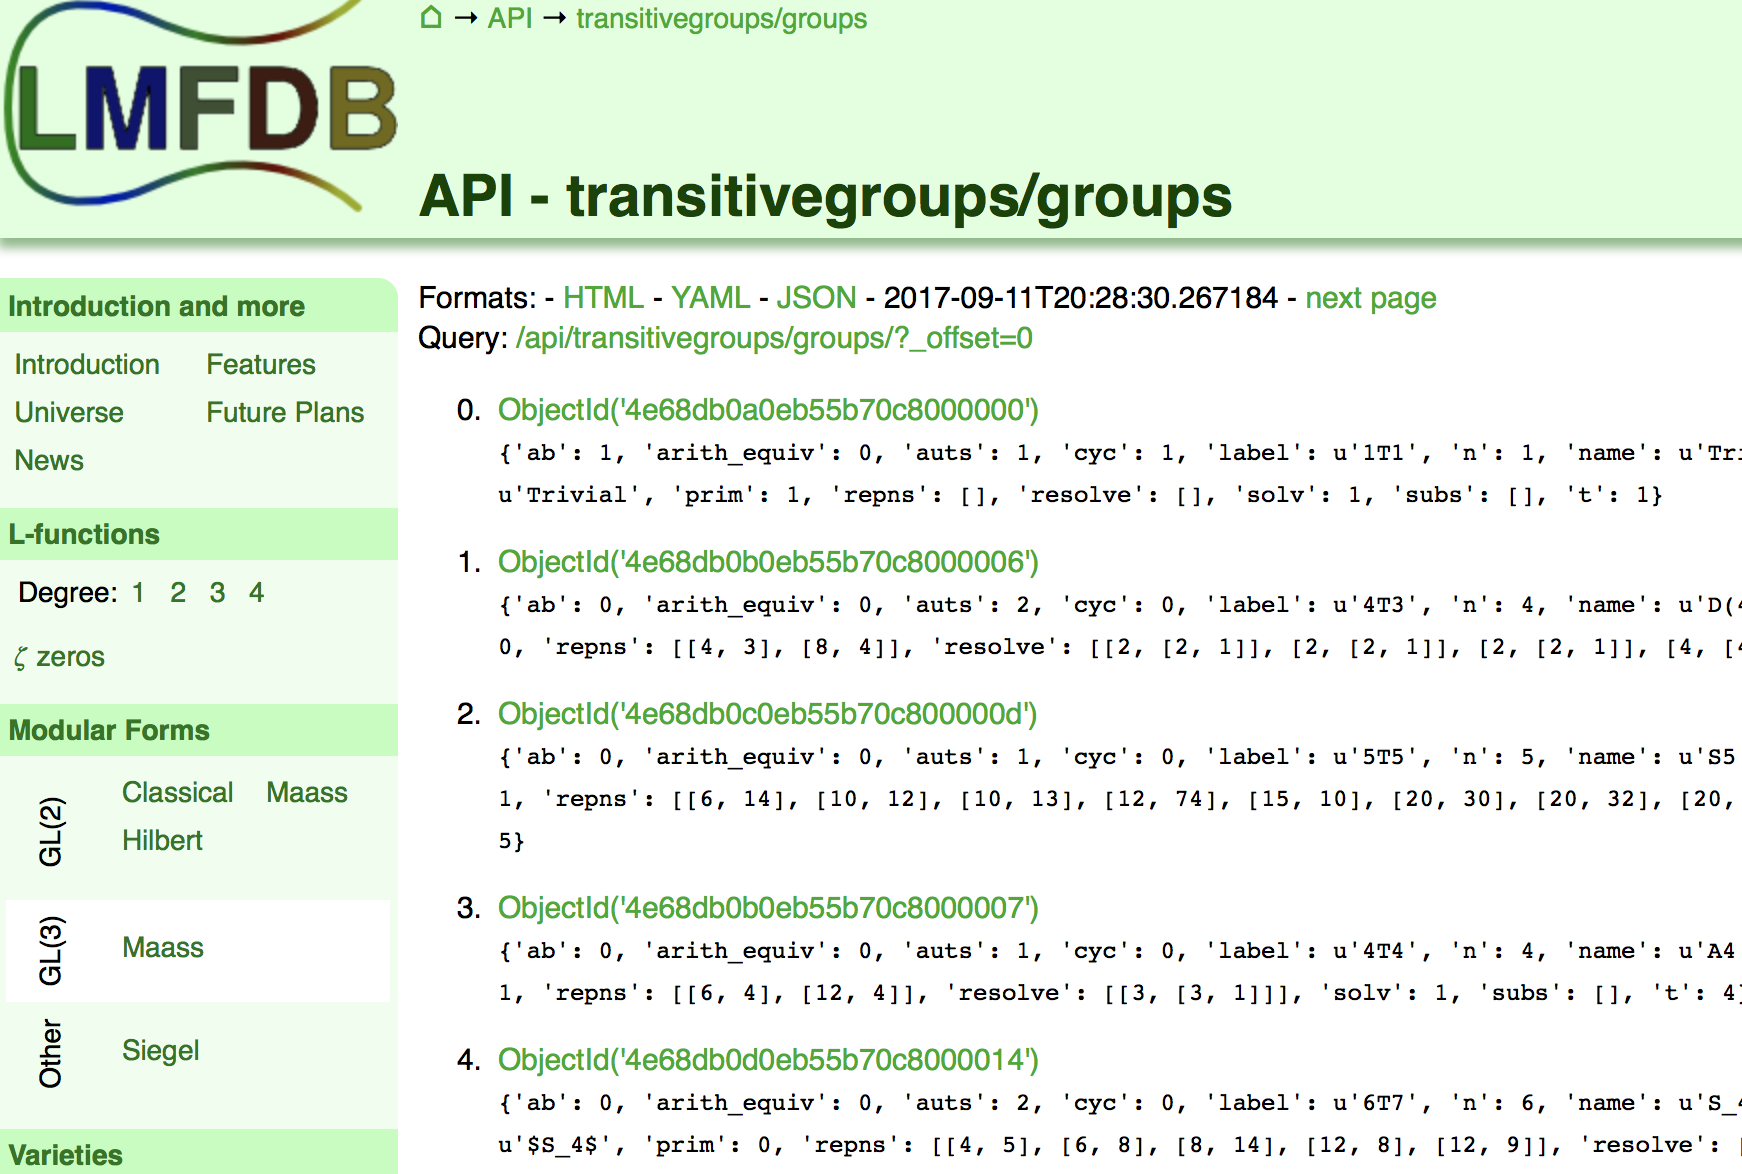
\includegraphics[width=0.97\textwidth,viewport=0 240 800 600 ,clip=true]{../MACIS17-vt/APIScreenshot}
  \caption{The Web-Interface for the \lmfdb API.}\label {fig:apiscreenshot}
\end{figure}

Queries must name the sub-database to be queried and consist of a set of key-value pairs that correspond to an SQL \texttt{where} clause.
However, while \lmfdb offers a programmable API for accessing its contents, this API sits at the level of the underlying MongoDB, and not the level of mathematical objects. 
For example, to retrieve all Abelian objects in the subdatabase of transitive groups, we expect to use the key-value pair \identifier{commutative}$ = $ \identifier{true}. 
However, these values need to be encoded to be understood by MongoDB.
We need to realize that the database schema actually uses the key \identifier{ab} for commutativity, that it has boolean values, and that the schema encodes \inlinecode{true} as \inlinecode{1}. 
Thus, the actual query to send is \url{http://www.lmfdb.org/api/transitivegroups/groups/?ab=1}. 

In this example, all steps are relatively straightforward. 
But in general, e.g. when searching for all elliptic curves with a specific isogeny matrix, this not only requires good familiarity with the mathematical background but also with the system internals of the particular \lmfdb sub-database; a skill set commonly found in neither research programmers nor average mathematicians.   

Our diagnosis is that {\lmfdb} -- and most other mathematical knowledge databases -- suffer from two problems:
\begin{compactitem}
\item \emph{human/computer mismatch}: humans have problems interacting with \lmfdb programmatically, because they must speak the system language instead of mathematical language
\item \emph{computer/computer mismatch}: mathematical computer systems cannot interoperate with \lmfdb without extending their code, because their system languages differ.
\end{compactitem}
Using the MitM approach we have presented in Section~\ref{sec:mmtmitm}, we can solve both problems at the same time by lifting the communication to the level of \ommt-encoded MitM objects, which both MitM-compatible software systems and humans can understand.
%%% Local Variables:
%%% mode: latex
%%% mode: visual-line
%%% fill-column: 5000
%%% TeX-master: "report"
%%% End:

%  LocalWords:  sec:sota lmfdb lmfdb lstlisting json ainvs iwp0 2adic_gens isogeny_matrix
%  LocalWords:  tamagawa_product 2adic_index anlist 4f71d4304d47869291435e6e vspace emph
%  LocalWords:  fig:lmfdbexample isogeny includegraphics textwidth fig:apiscreenshot
%  LocalWords:  centering summarize sec:mmtmitm ommt-encoded 4f71d4304d47869291435e6e
%  LocalWords:  serialization wrapfigure
